\newcommand{\vinSection}[2][\newpage]{%
	#1
	\fancyhead[LE]{\bfseries\nouppercase{\leftmark}}      % Chapter in the right on even pages
	\fancyhead[RO]{\bfseries\nouppercase{\leftmark}}      % Chapter in the right on even pages
	\fancyhead[LO]{\bfseries\nouppercase{\rightmark}}      % Chapter in the right on even pages
	\fancyhead[RE]{\bfseries\nouppercase{\rightmark}}      % Chapter in the right on even pages
	%\lhead{\leftmark}%
    \chead{}%
    %\rhead{\rightmark}%
    \lfoot{}%
    \rfoot{}%
    \subsubsection{#2}%
}


\newcommand{\vinShowInfoDomain}[3]{
	\noindent
	\begin{minipage}[t]{\textwidth}
	\vspace{0pt}
		\begin{tabular}{l p{7.5cm} }
		Producteur:     & {#1}\\
		Adresse:        & {#2}\\
	\end{tabular}
	\end{minipage}		
	\par
	\hfill
	\vspace{2pt}
	\begin{figure}[!h]
		\includegraphics[width=\textwidth]{#3}
	\end{figure}
	}
\newcommand{\vinShowCouleur}[1]{
	\noindent
	\begin{minipage}[t]{.3\textwidth}
	%\begin{tcolorbox}[width=.3\textwidth,]
		{\color{orangecolor}\textbf{#1}}
	%\end{tcolorbox}
	\end{minipage}	
	\hfill
	\vspace{6pt}
	}

\newcommand{\vinShowInfoAppellation}[3]{
	\noindent
	\begin{minipage}[t]{\textwidth}
	{\textbf{#1}}%
	\vspace{1pt}
	\end{minipage}		
	\begin{minipage}[t]{\textwidth}
		\begin{tabular}{l p{7.5cm} }
		Cuv\'ee :    & {#2}\\ 
		C\'epage:    & {#3}\\
	\end{tabular}
	\end{minipage}		
	}

\setlength{\ellipsisgap}{0.02em}

%%%%%%%%%%%%%%%%%%%%%%%%%%%%%%%%%%%

\newpage 
\fancyhead[LE]{\bfseries\nouppercase{\leftmark} } 
\fancyhead[RO]{\bfseries\nouppercase{\leftmark} } 
\fancyhead[LO]{\bfseries\nouppercase{\rightmark} }
\fancyhead[RE]{\bfseries\nouppercase{\rightmark} }

\section{Au Sujet des Vins}
\addthumb{Au Sujet des Vins}{\thumbsIcon}{white}{darkraspberry}

blablabla

les vins sont ranges par bassin. Chaque bassin est symbolisées par une icônes qui apparait dans la marque de couleur suivant la forme du verre associe au vin.
\medskip
{\renewcommand{\arraystretch}{1.7}
\begin{center}
\begin{tabular}{ l l l l }
\setbox0=\hbox{\put(0,0){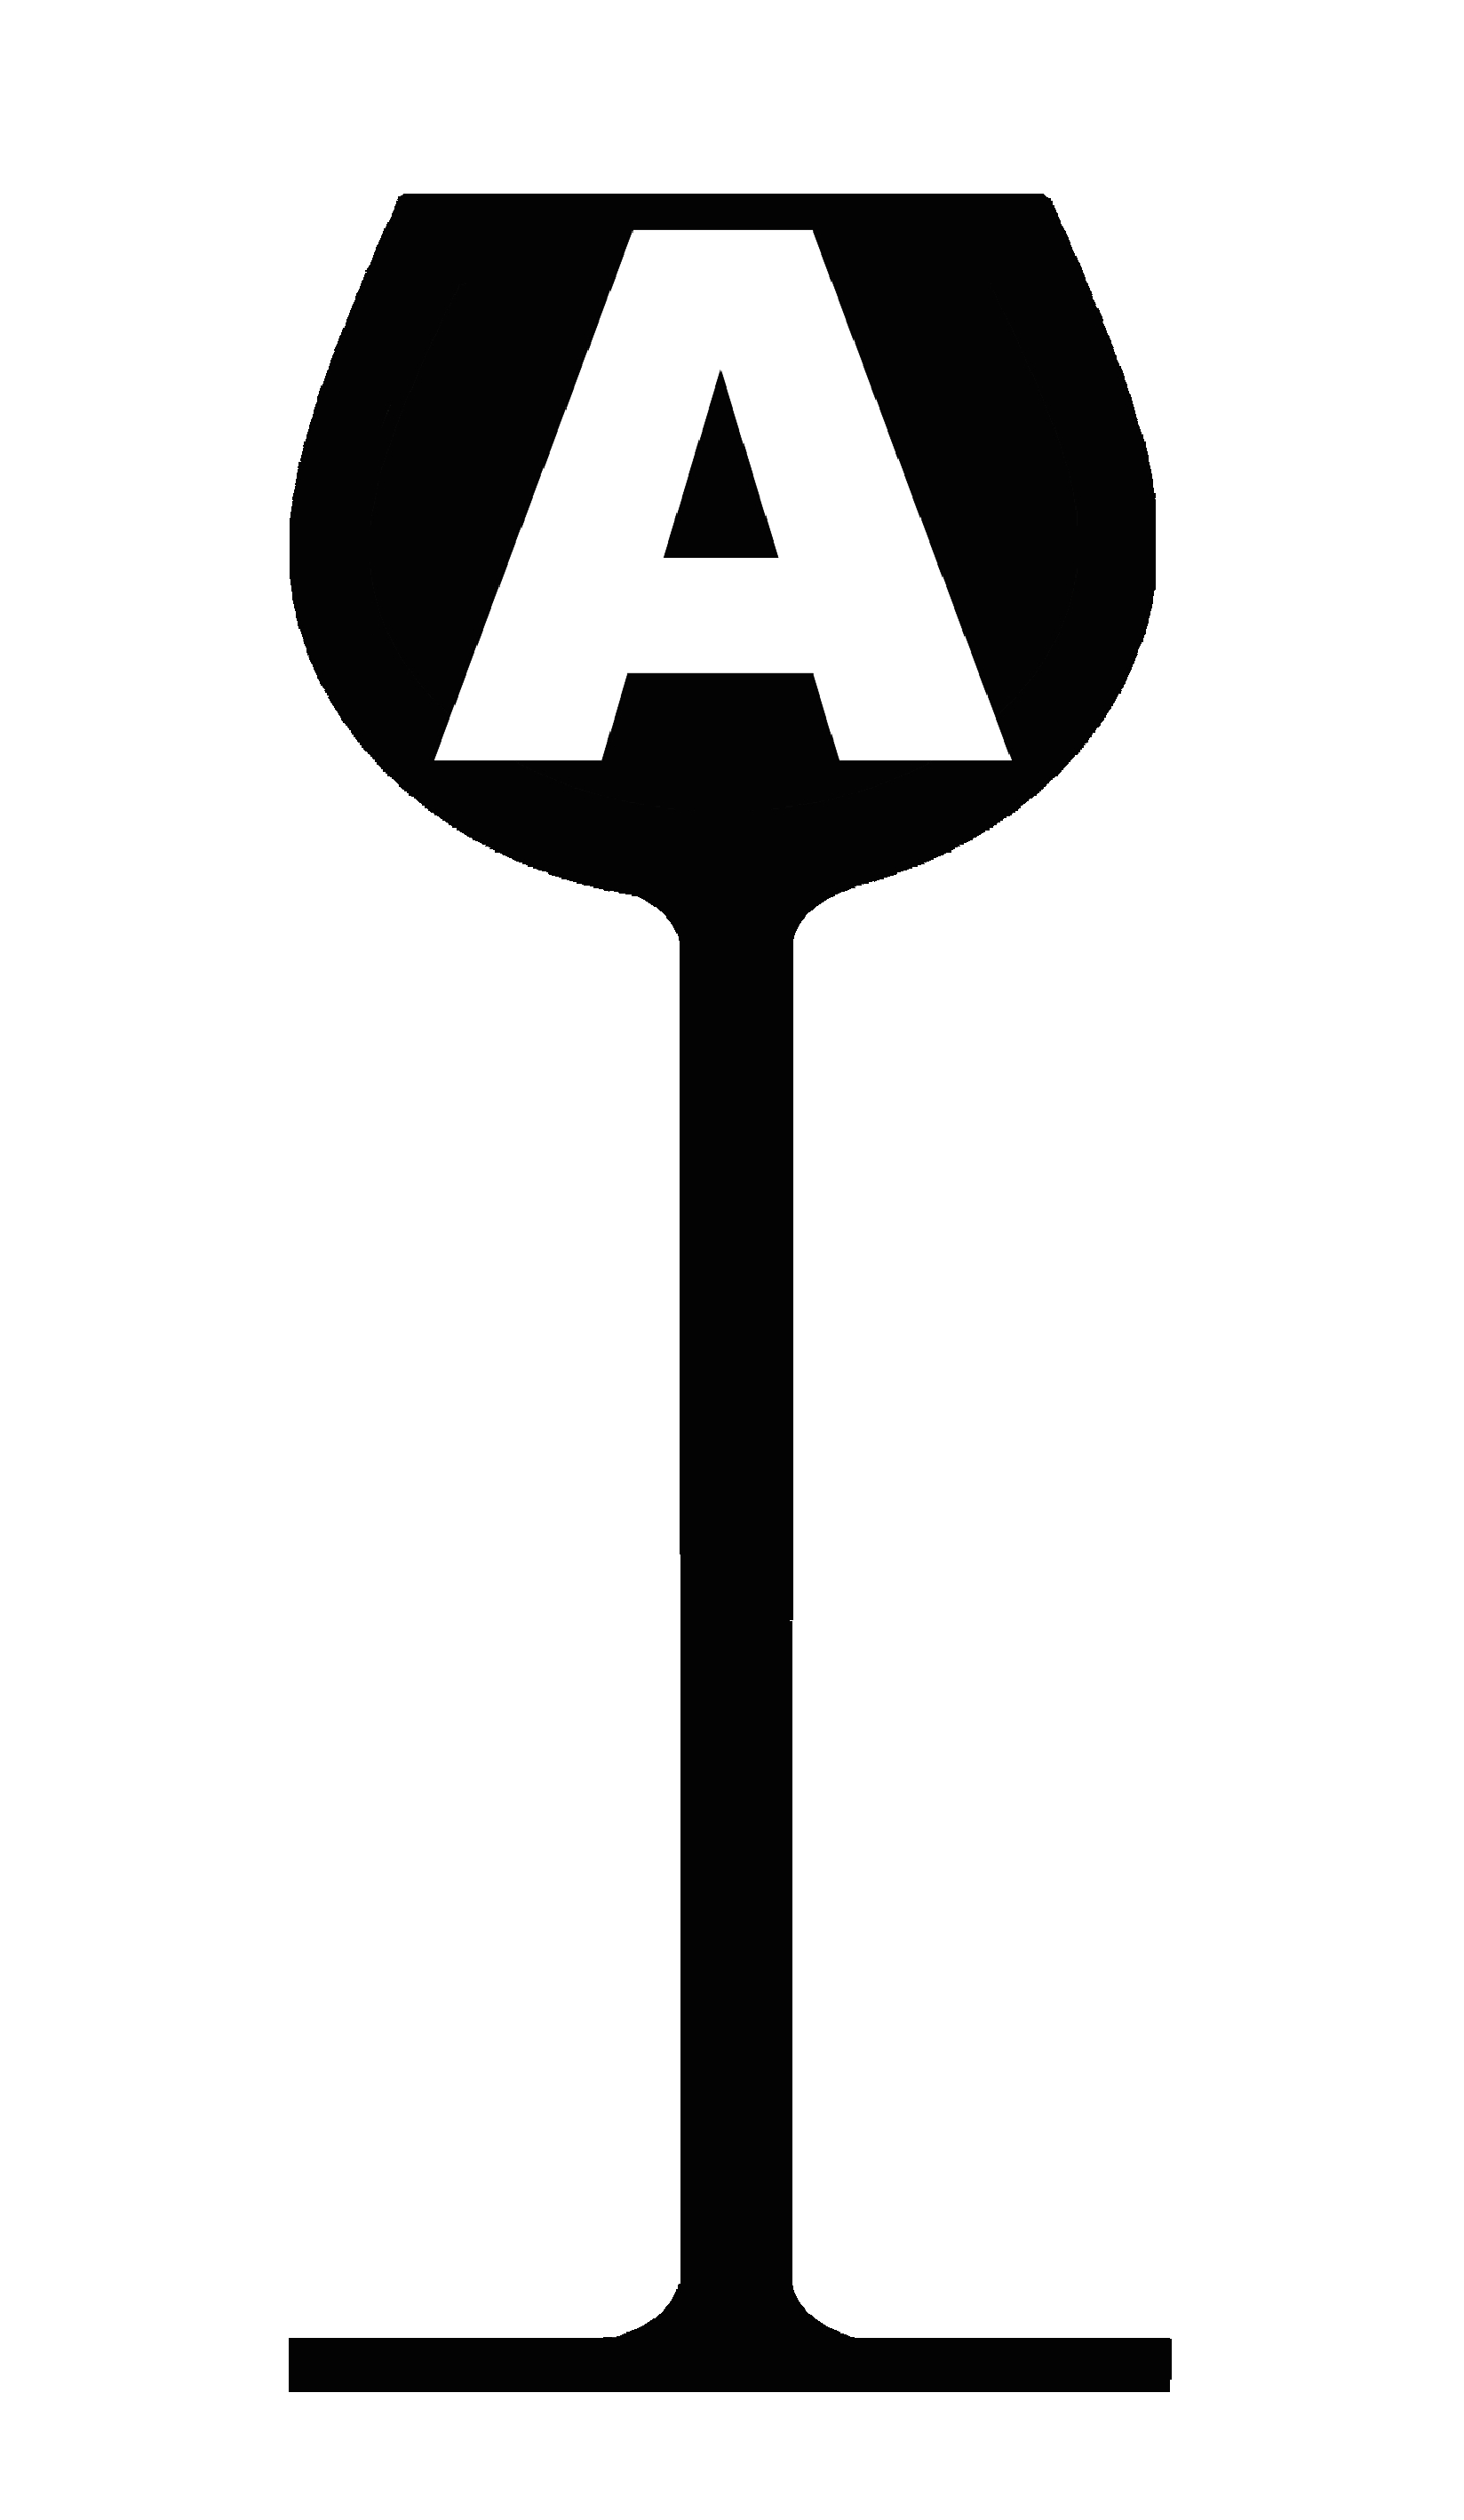
\includegraphics[scale=0.021, trim= 0em -5em -5em -5em,]{Icones/icon_alsace_black.pdf}}}
	\parbox{\wd0}{\box0} 
	& \quad Alsace  & 
\setbox0=\hbox{\put(0,0){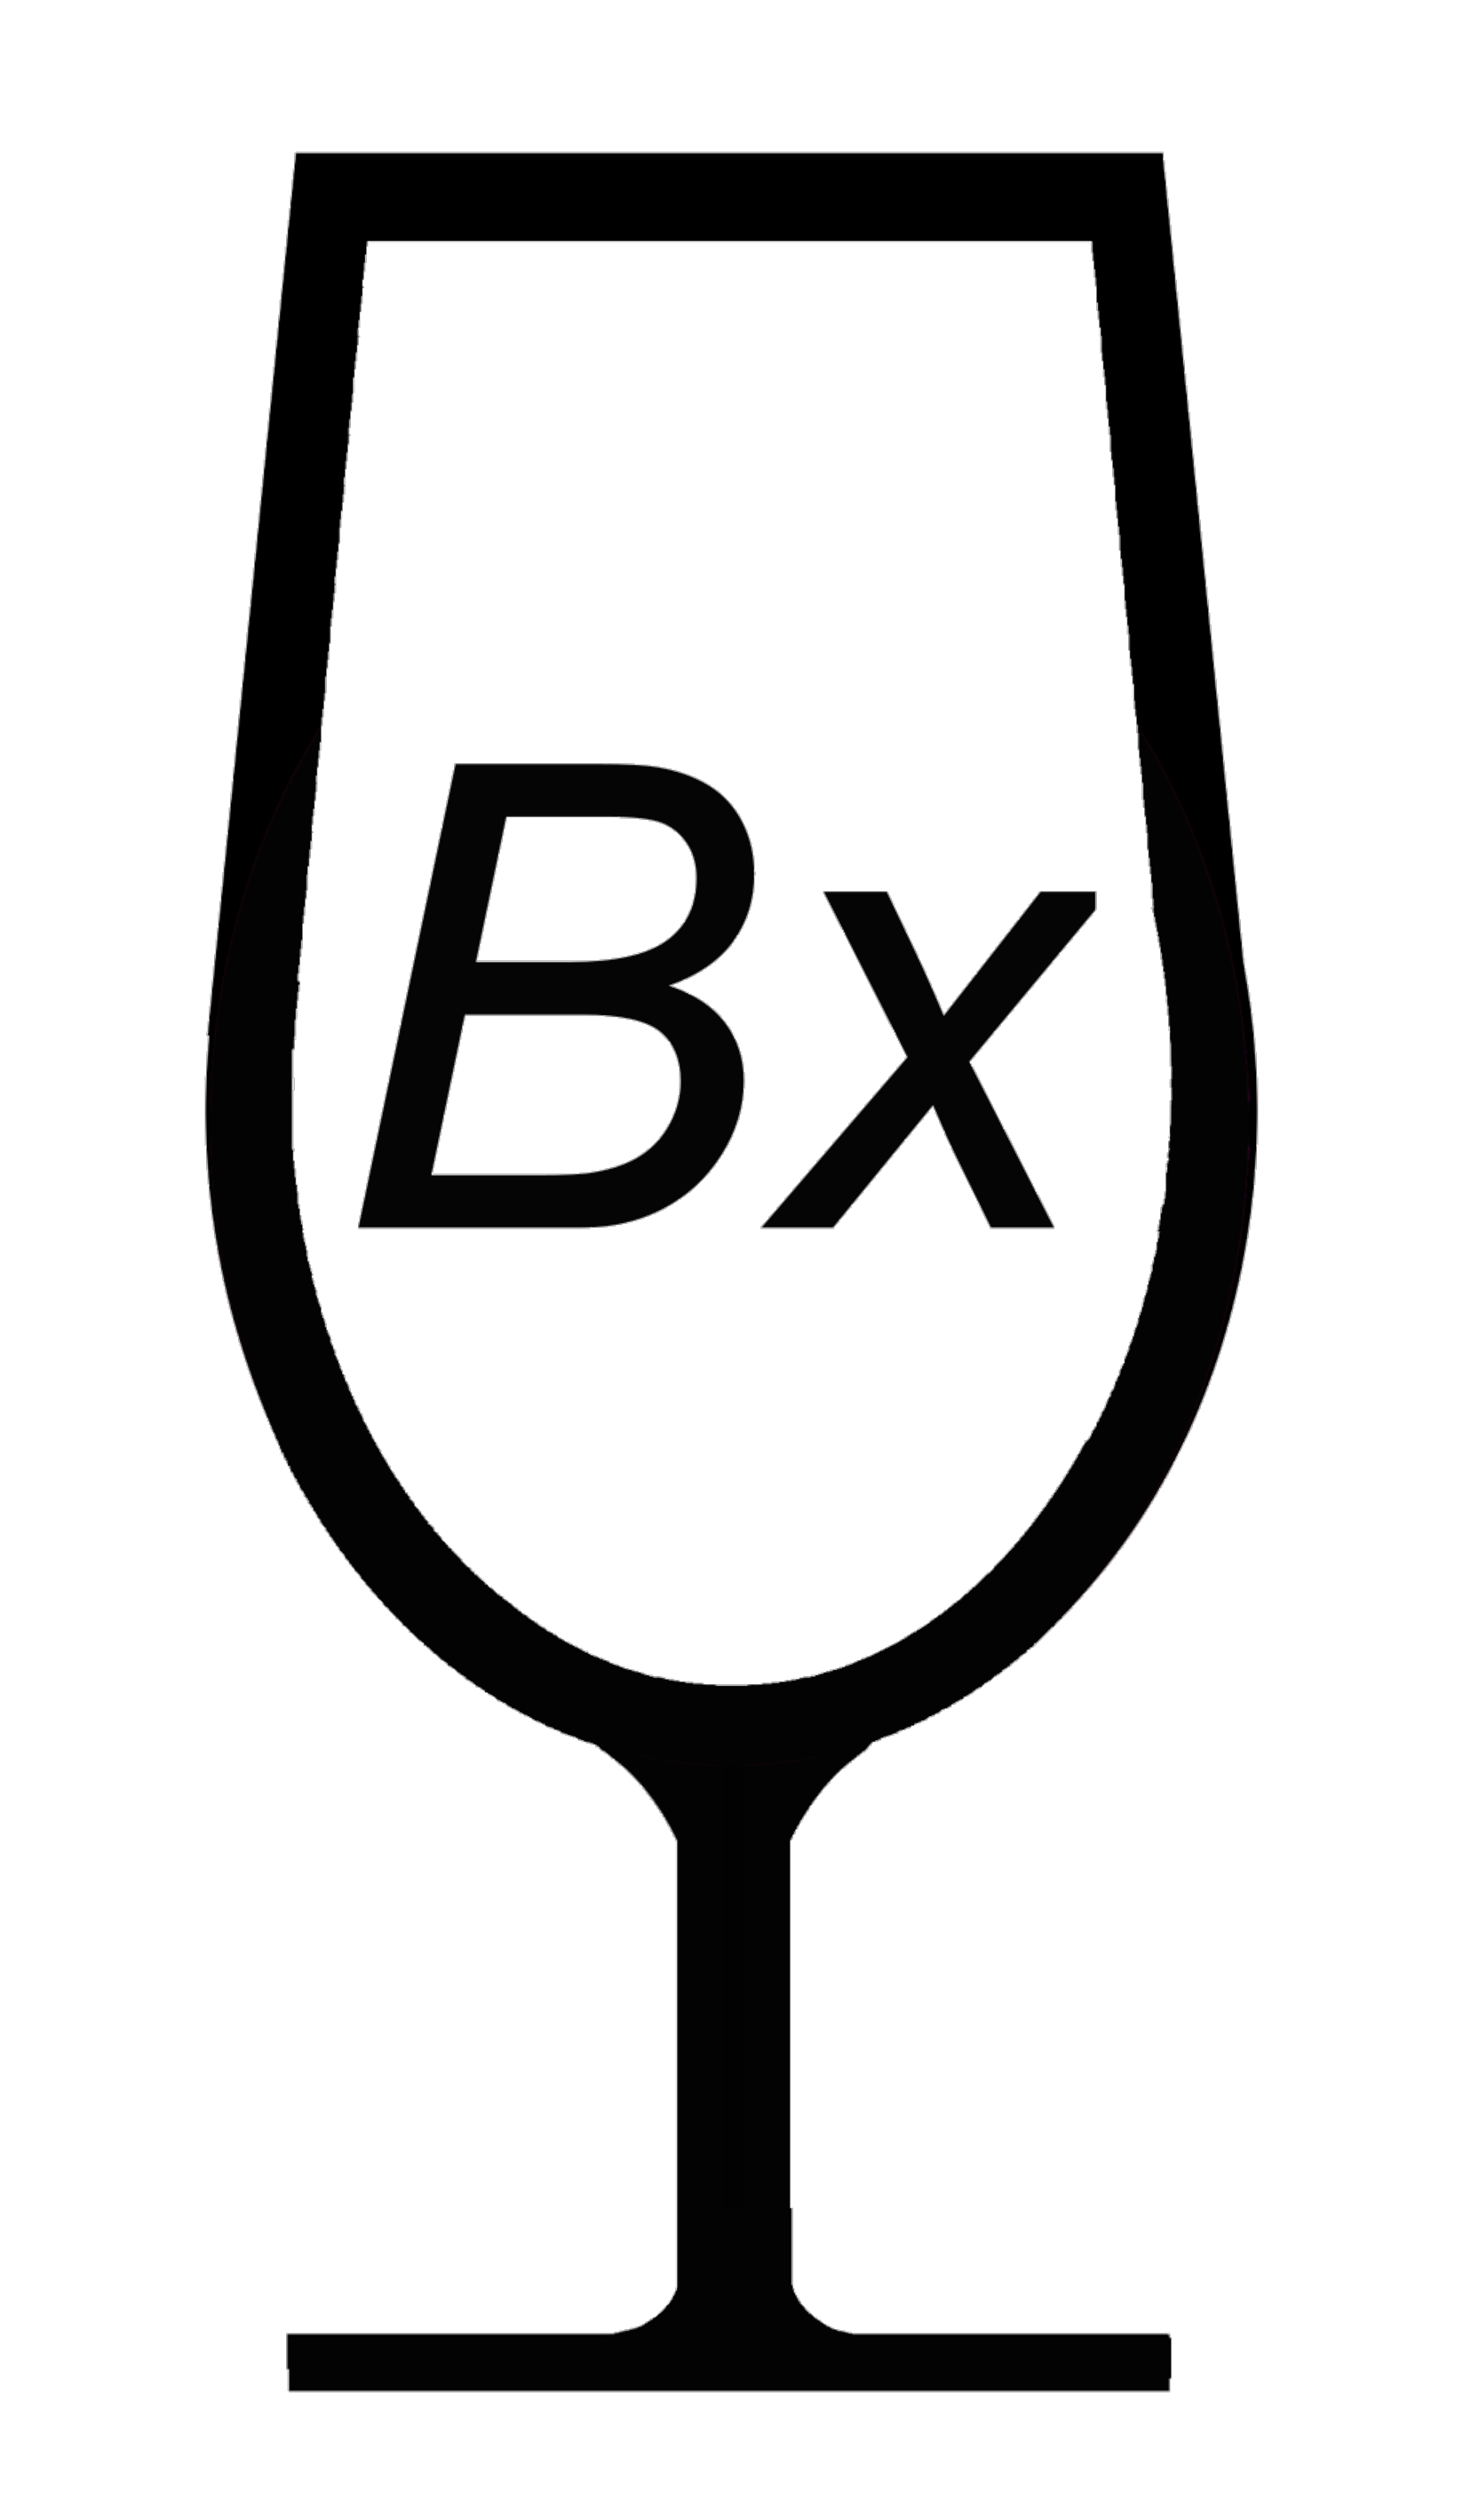
\includegraphics[scale=0.021, trim= 0em -5em -5em -5em,]{Icones/icon_bordeaux_black.pdf}}}
	\parbox{\wd0}{\box0}
	& \quad Bordeaux  \\ 
\setbox0=\hbox{\put(0,0){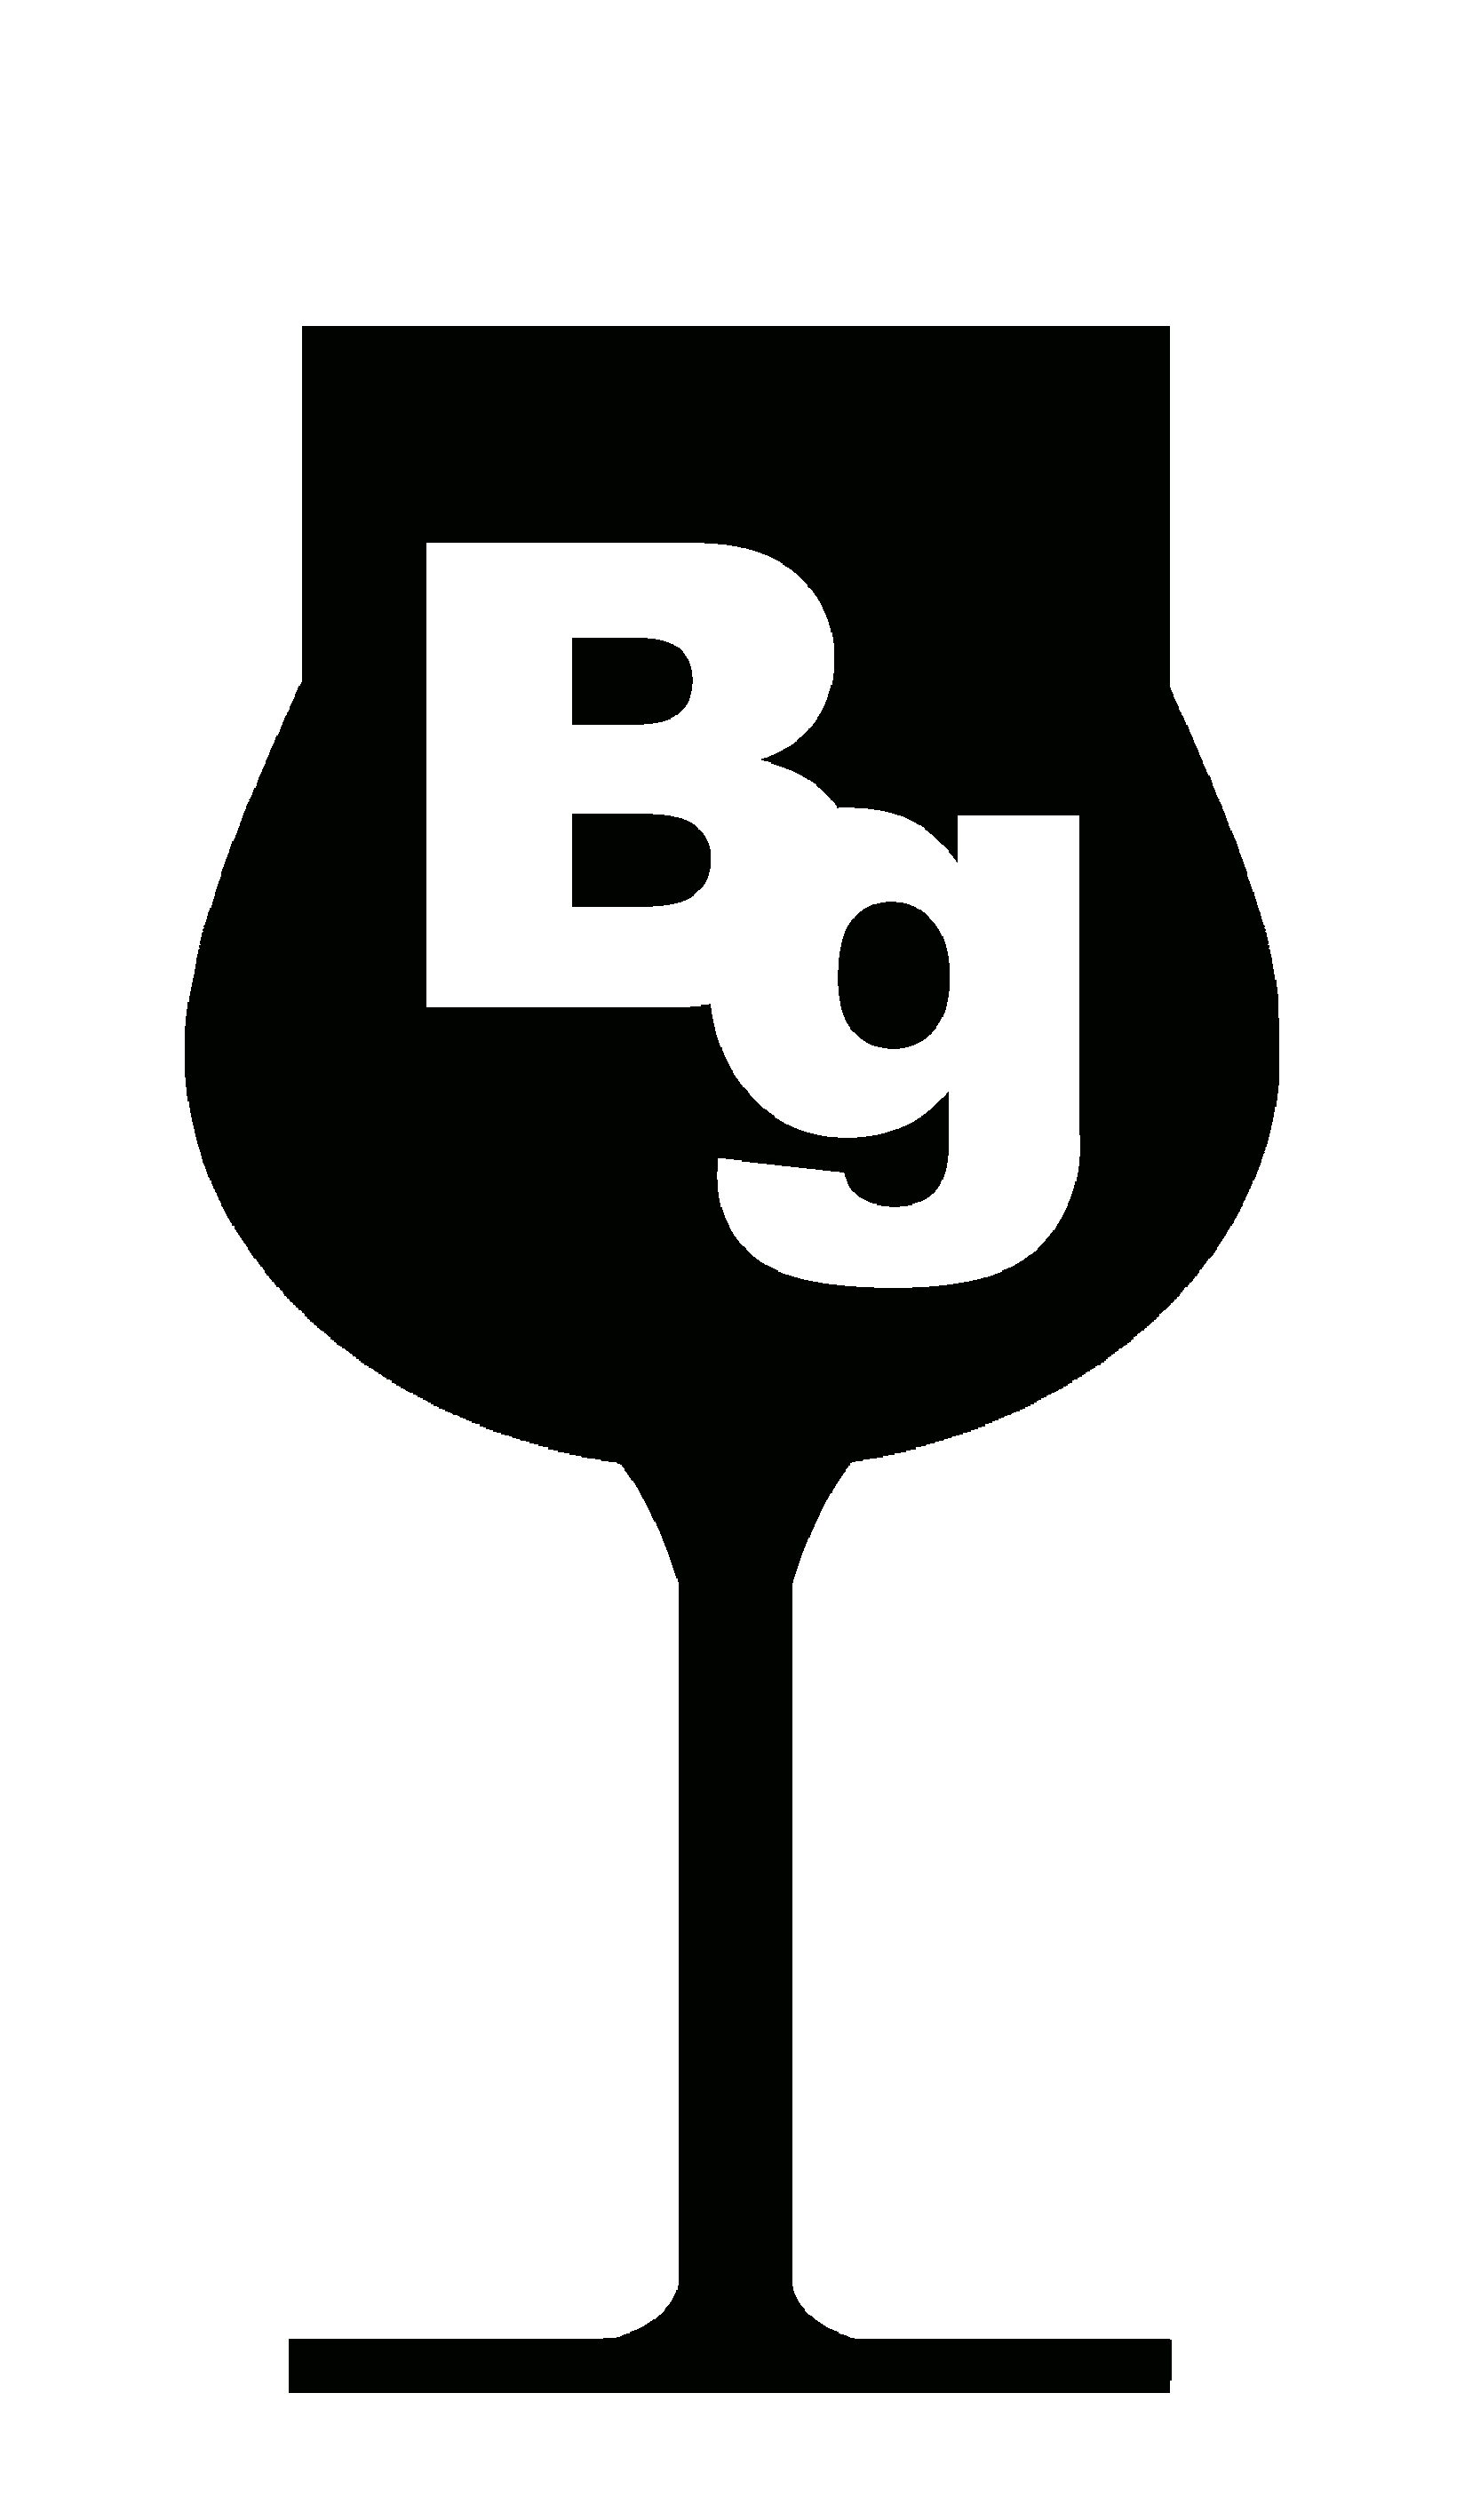
\includegraphics[scale=0.021, trim= 0em -5em -5em -5em,]{Icones/icon_bourgogne_black.pdf}}}
	\parbox{\wd0}{\box0}
	& \quad Bourgogne  & 
\setbox0=\hbox{\put(0,0){
\includegraphics[scale=0.021, trim= 0em -5em -5em -5em,]{Icones/icon_champagne_black.pdf}}}
	\parbox{\wd0}{\box0}
	& \quad Champagne  \\ 
\setbox0=\hbox{\put(0,0){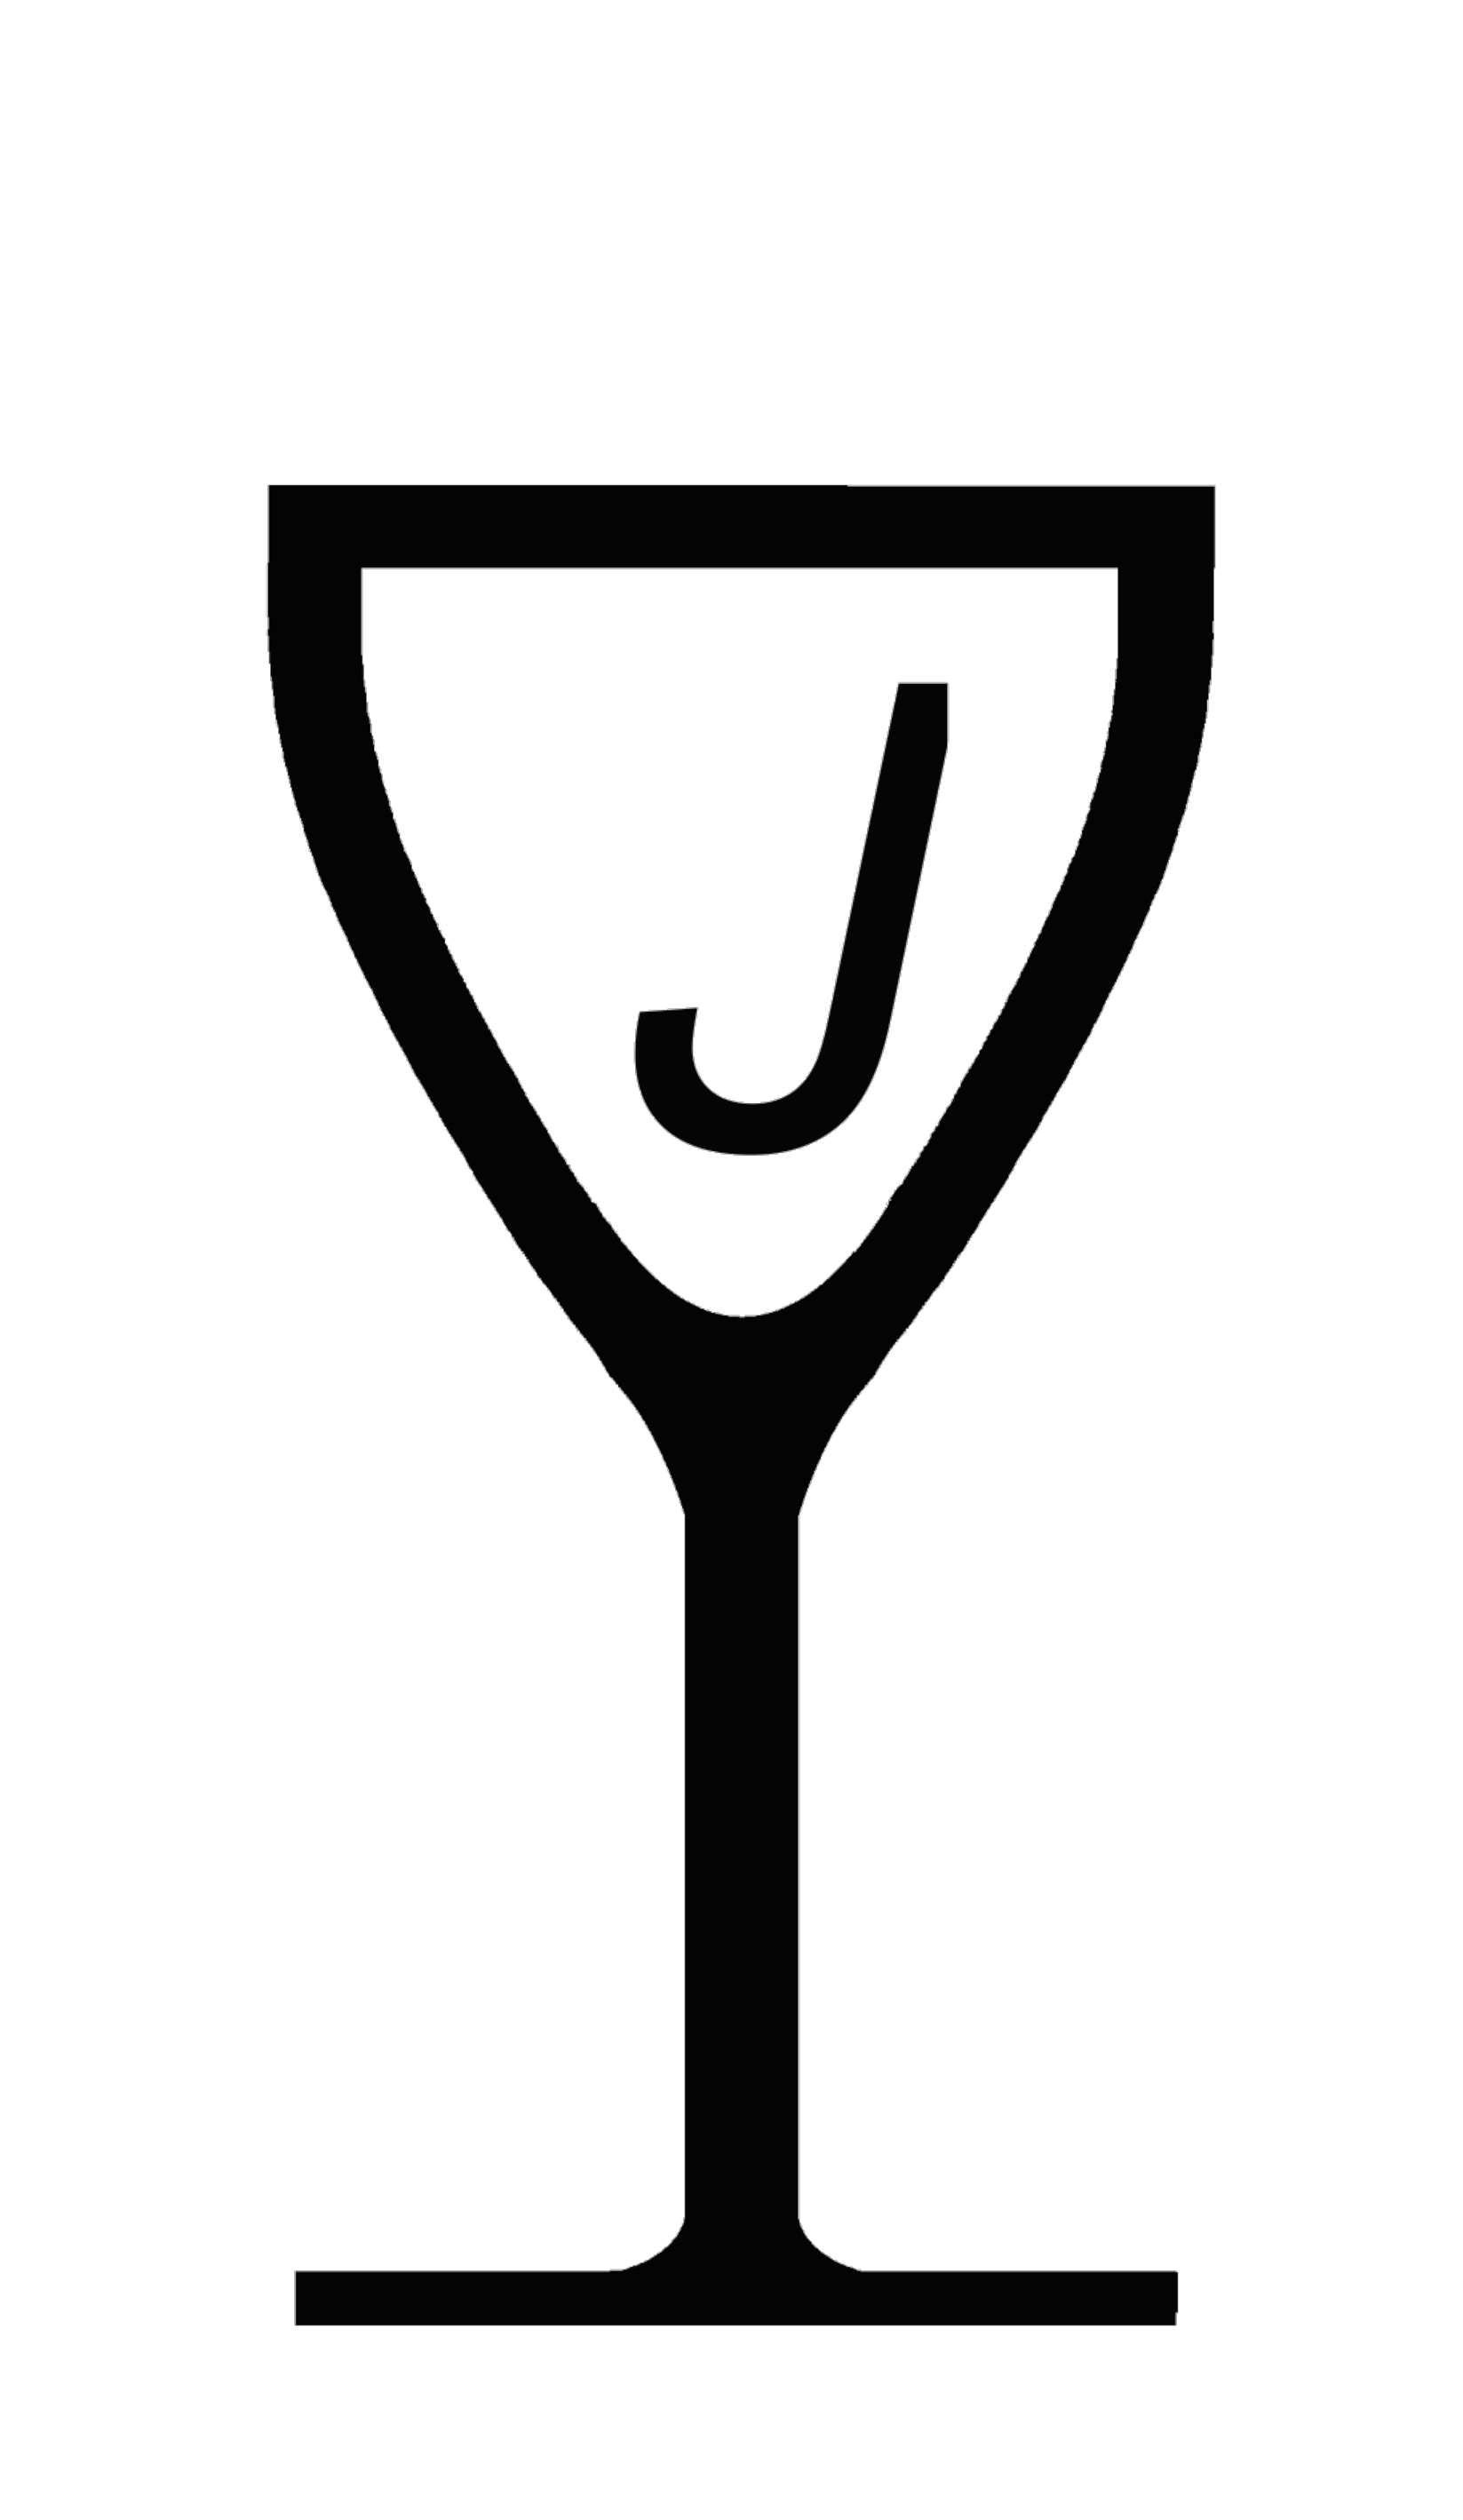
\includegraphics[scale=0.021, trim= 0em -5em -5em -5em,]{Icones/icon_jura_black.pdf}}}
	\parbox{\wd0}{\box0}
	& \quad Jura  & 
\setbox0=\hbox{\put(0,0){
\includegraphics[scale=0.021, trim= 0em -5em -5em -5em,]{Icones/icon_languedoc_black.pdf}}}
	\parbox{\wd0}{\box0}
	& \quad Languedoc-Rousillon  \\ 
\setbox0=\hbox{\put(0,0){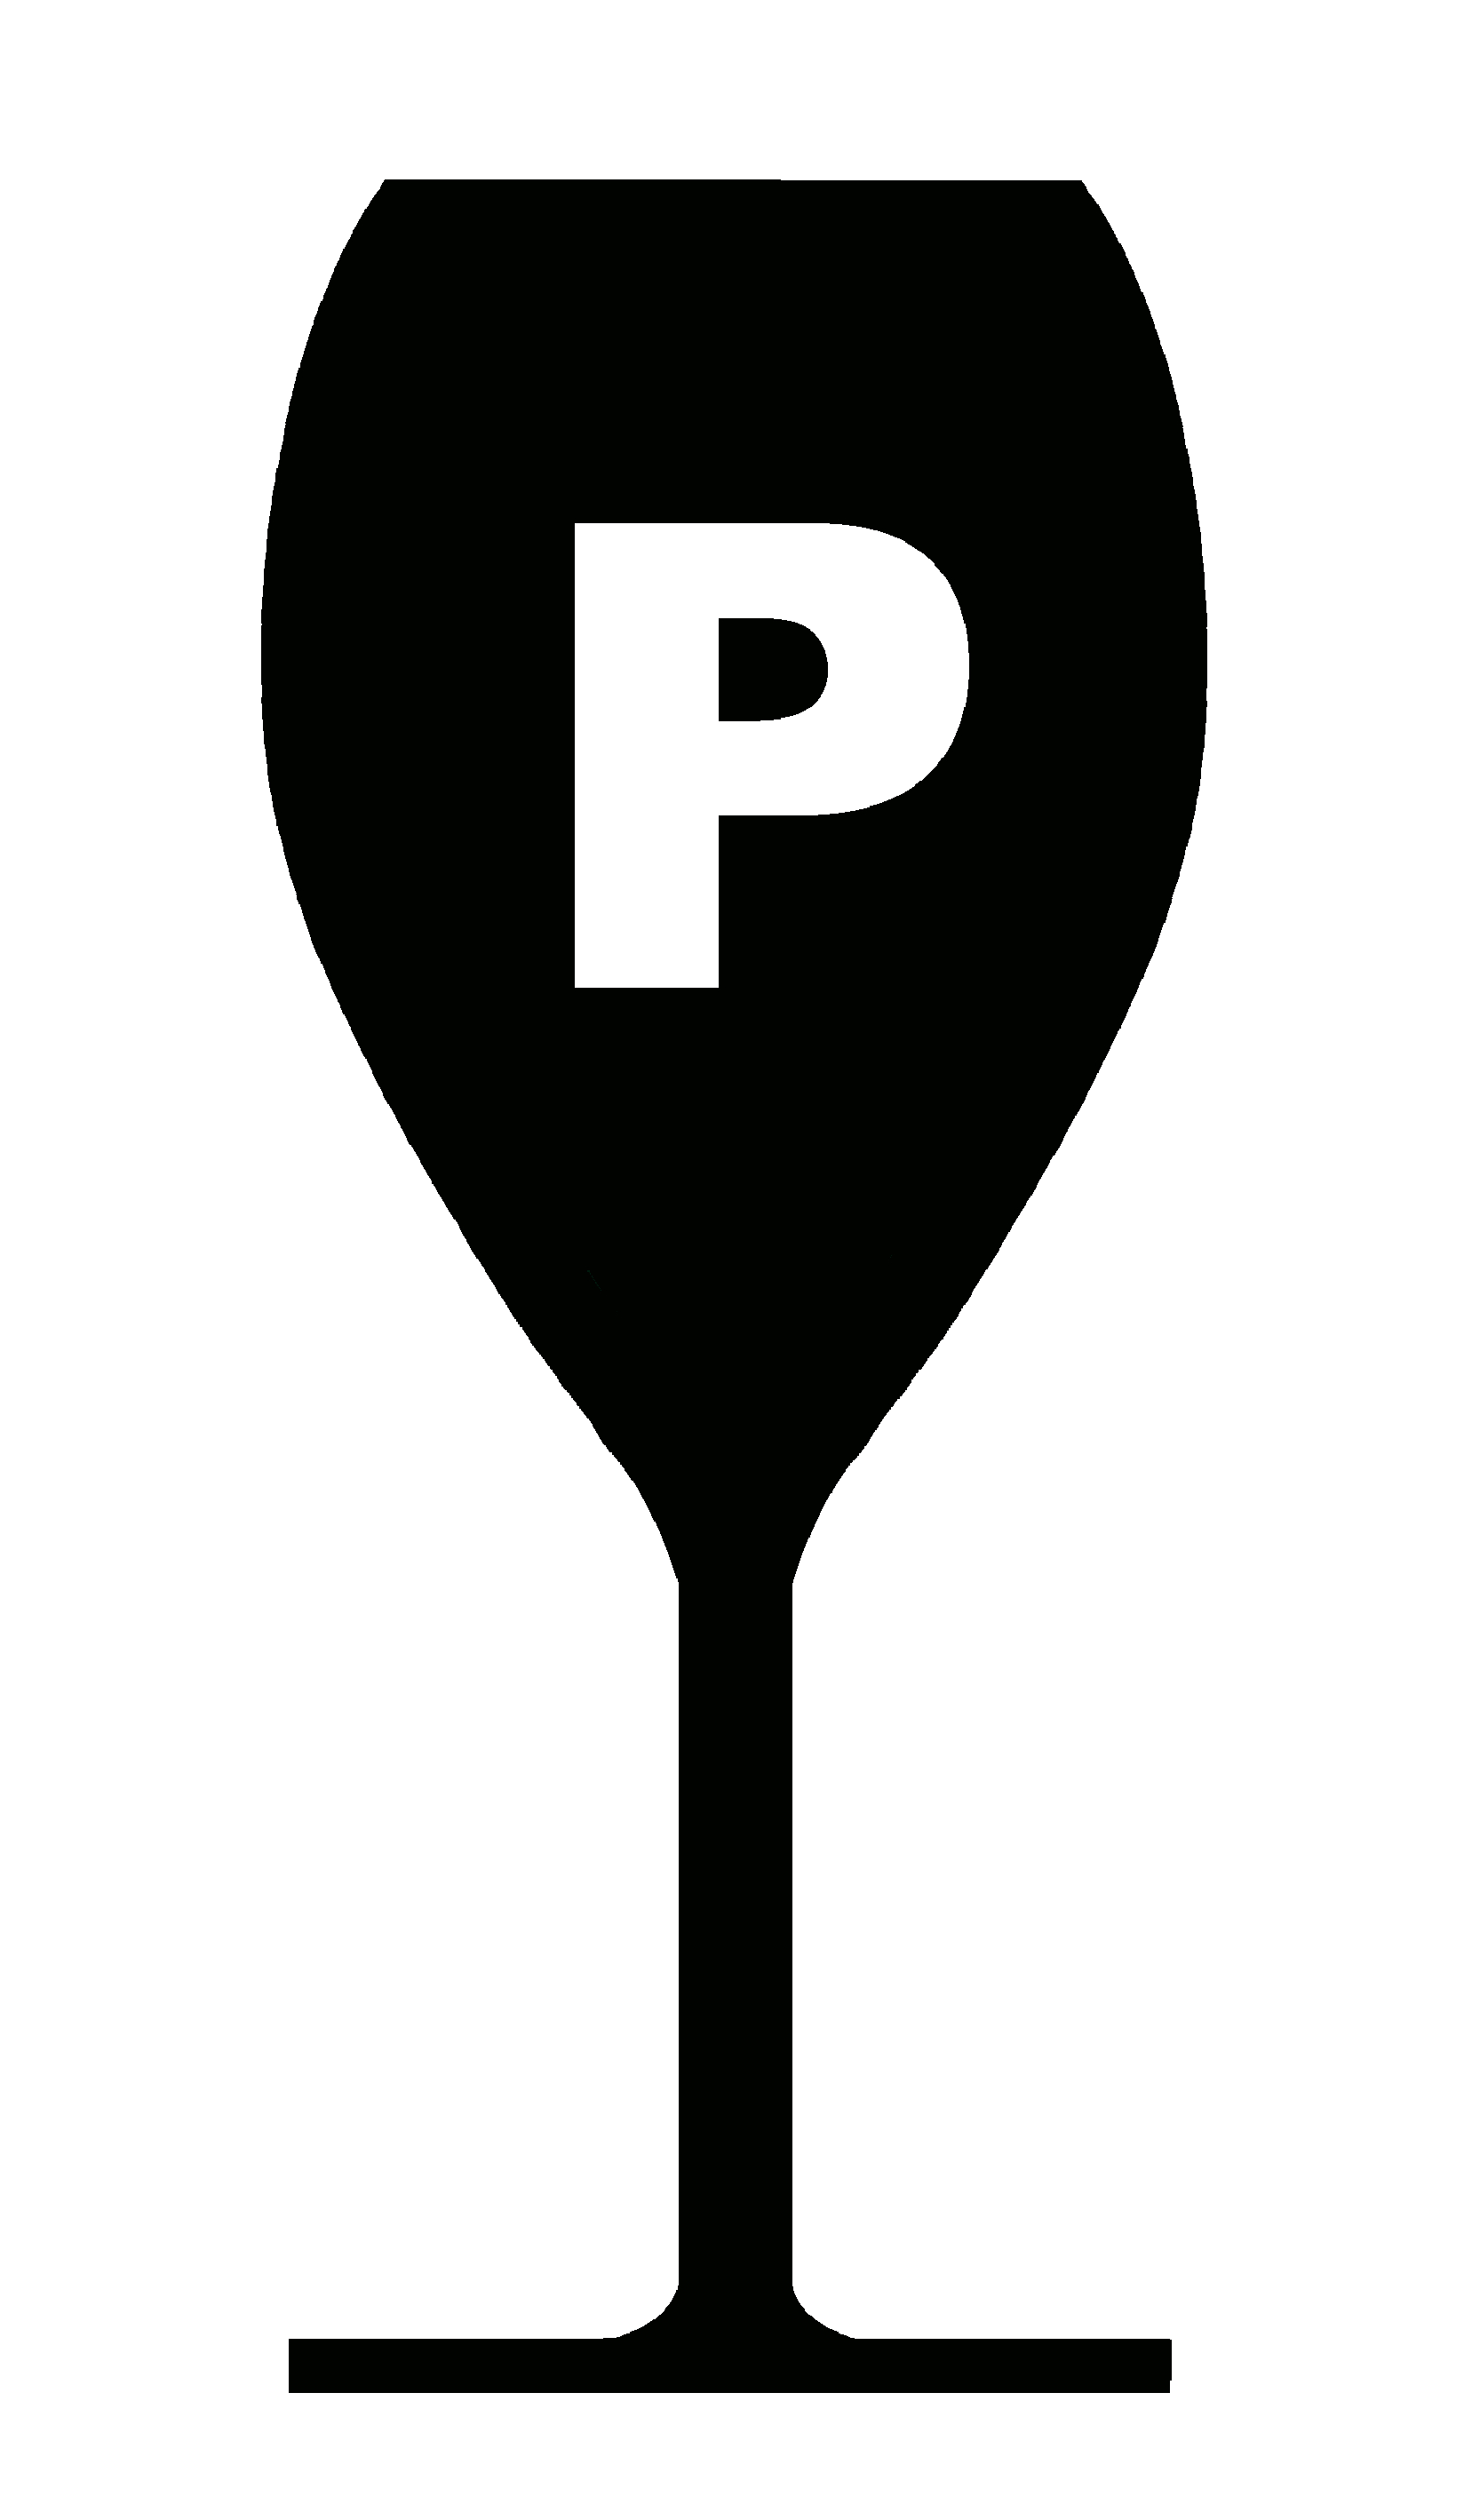
\includegraphics[scale=0.021, trim= 0em -5em -5em -5em,]{Icones/icon_provence_black.pdf}}}
	\parbox{\wd0}{\box0}
	& \quad Provence  & 
\setbox0=\hbox{\put(0,0){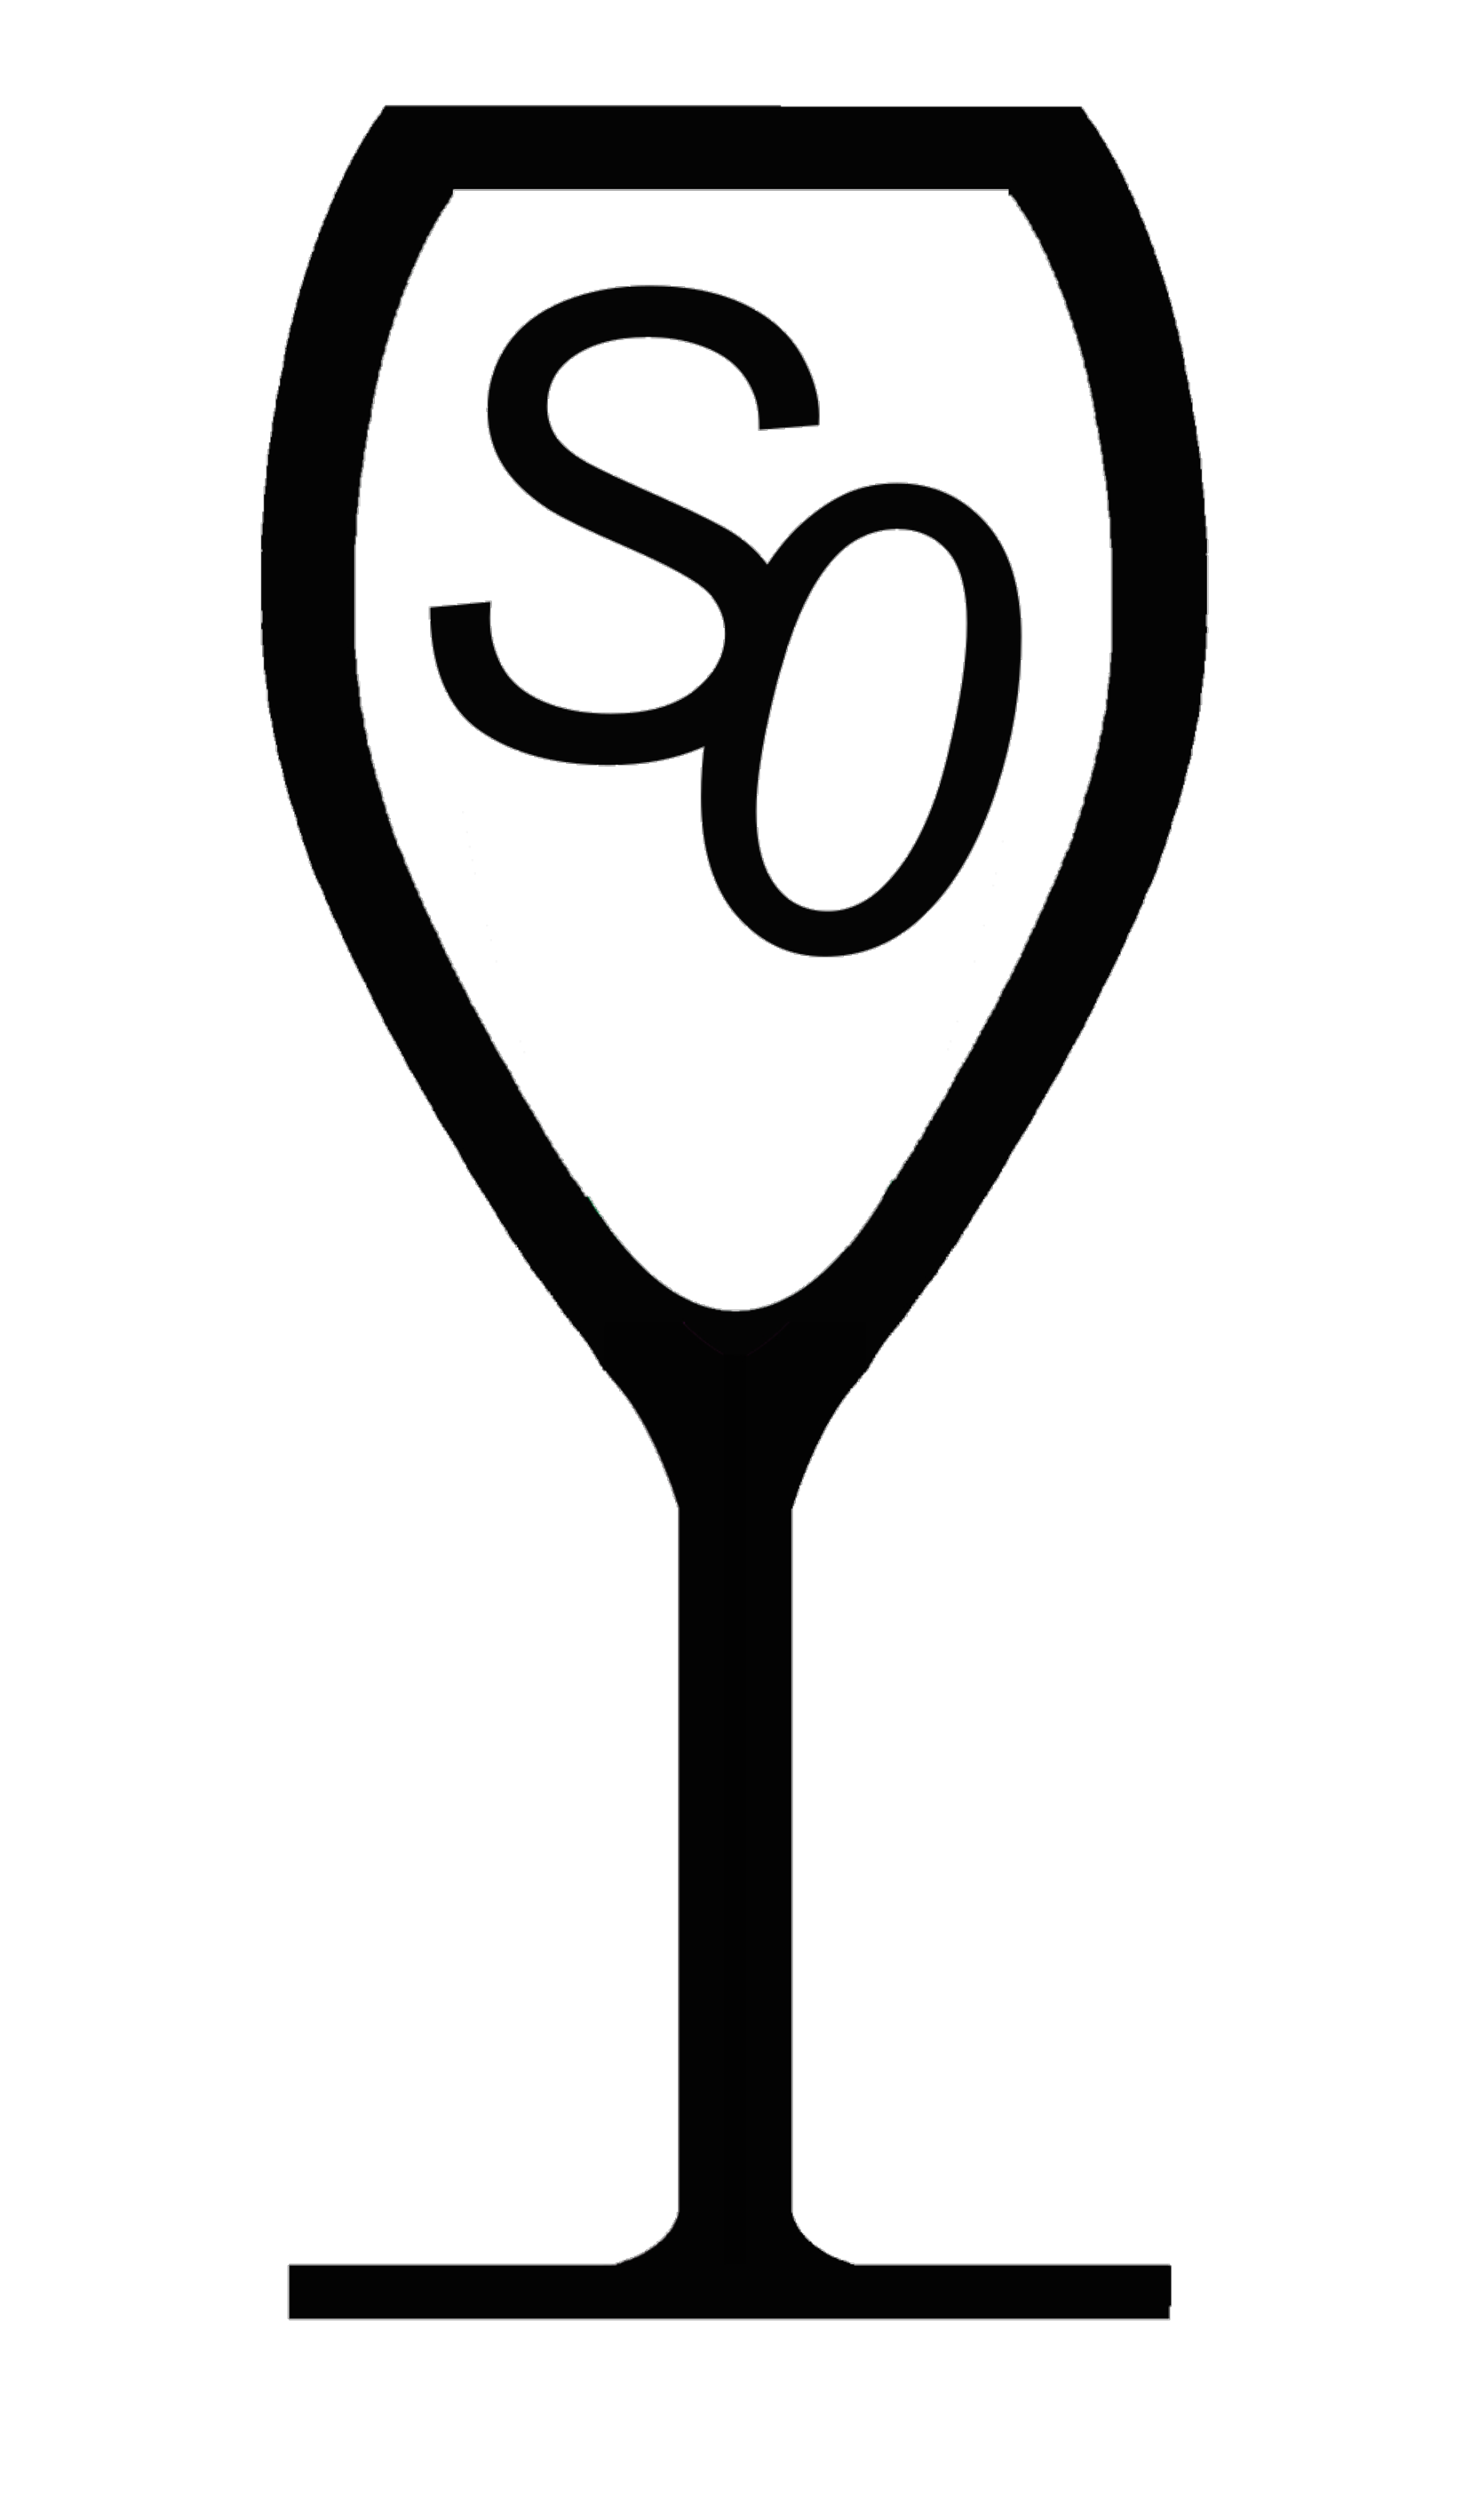
\includegraphics[scale=0.021, trim= 0em -5em -5em -5em,]{Icones/icon_sudouest_black.pdf}}}
	\parbox{\wd0}{\box0}
	& \quad Sud-Ouest \\ 
\setbox0=\hbox{\put(0,0){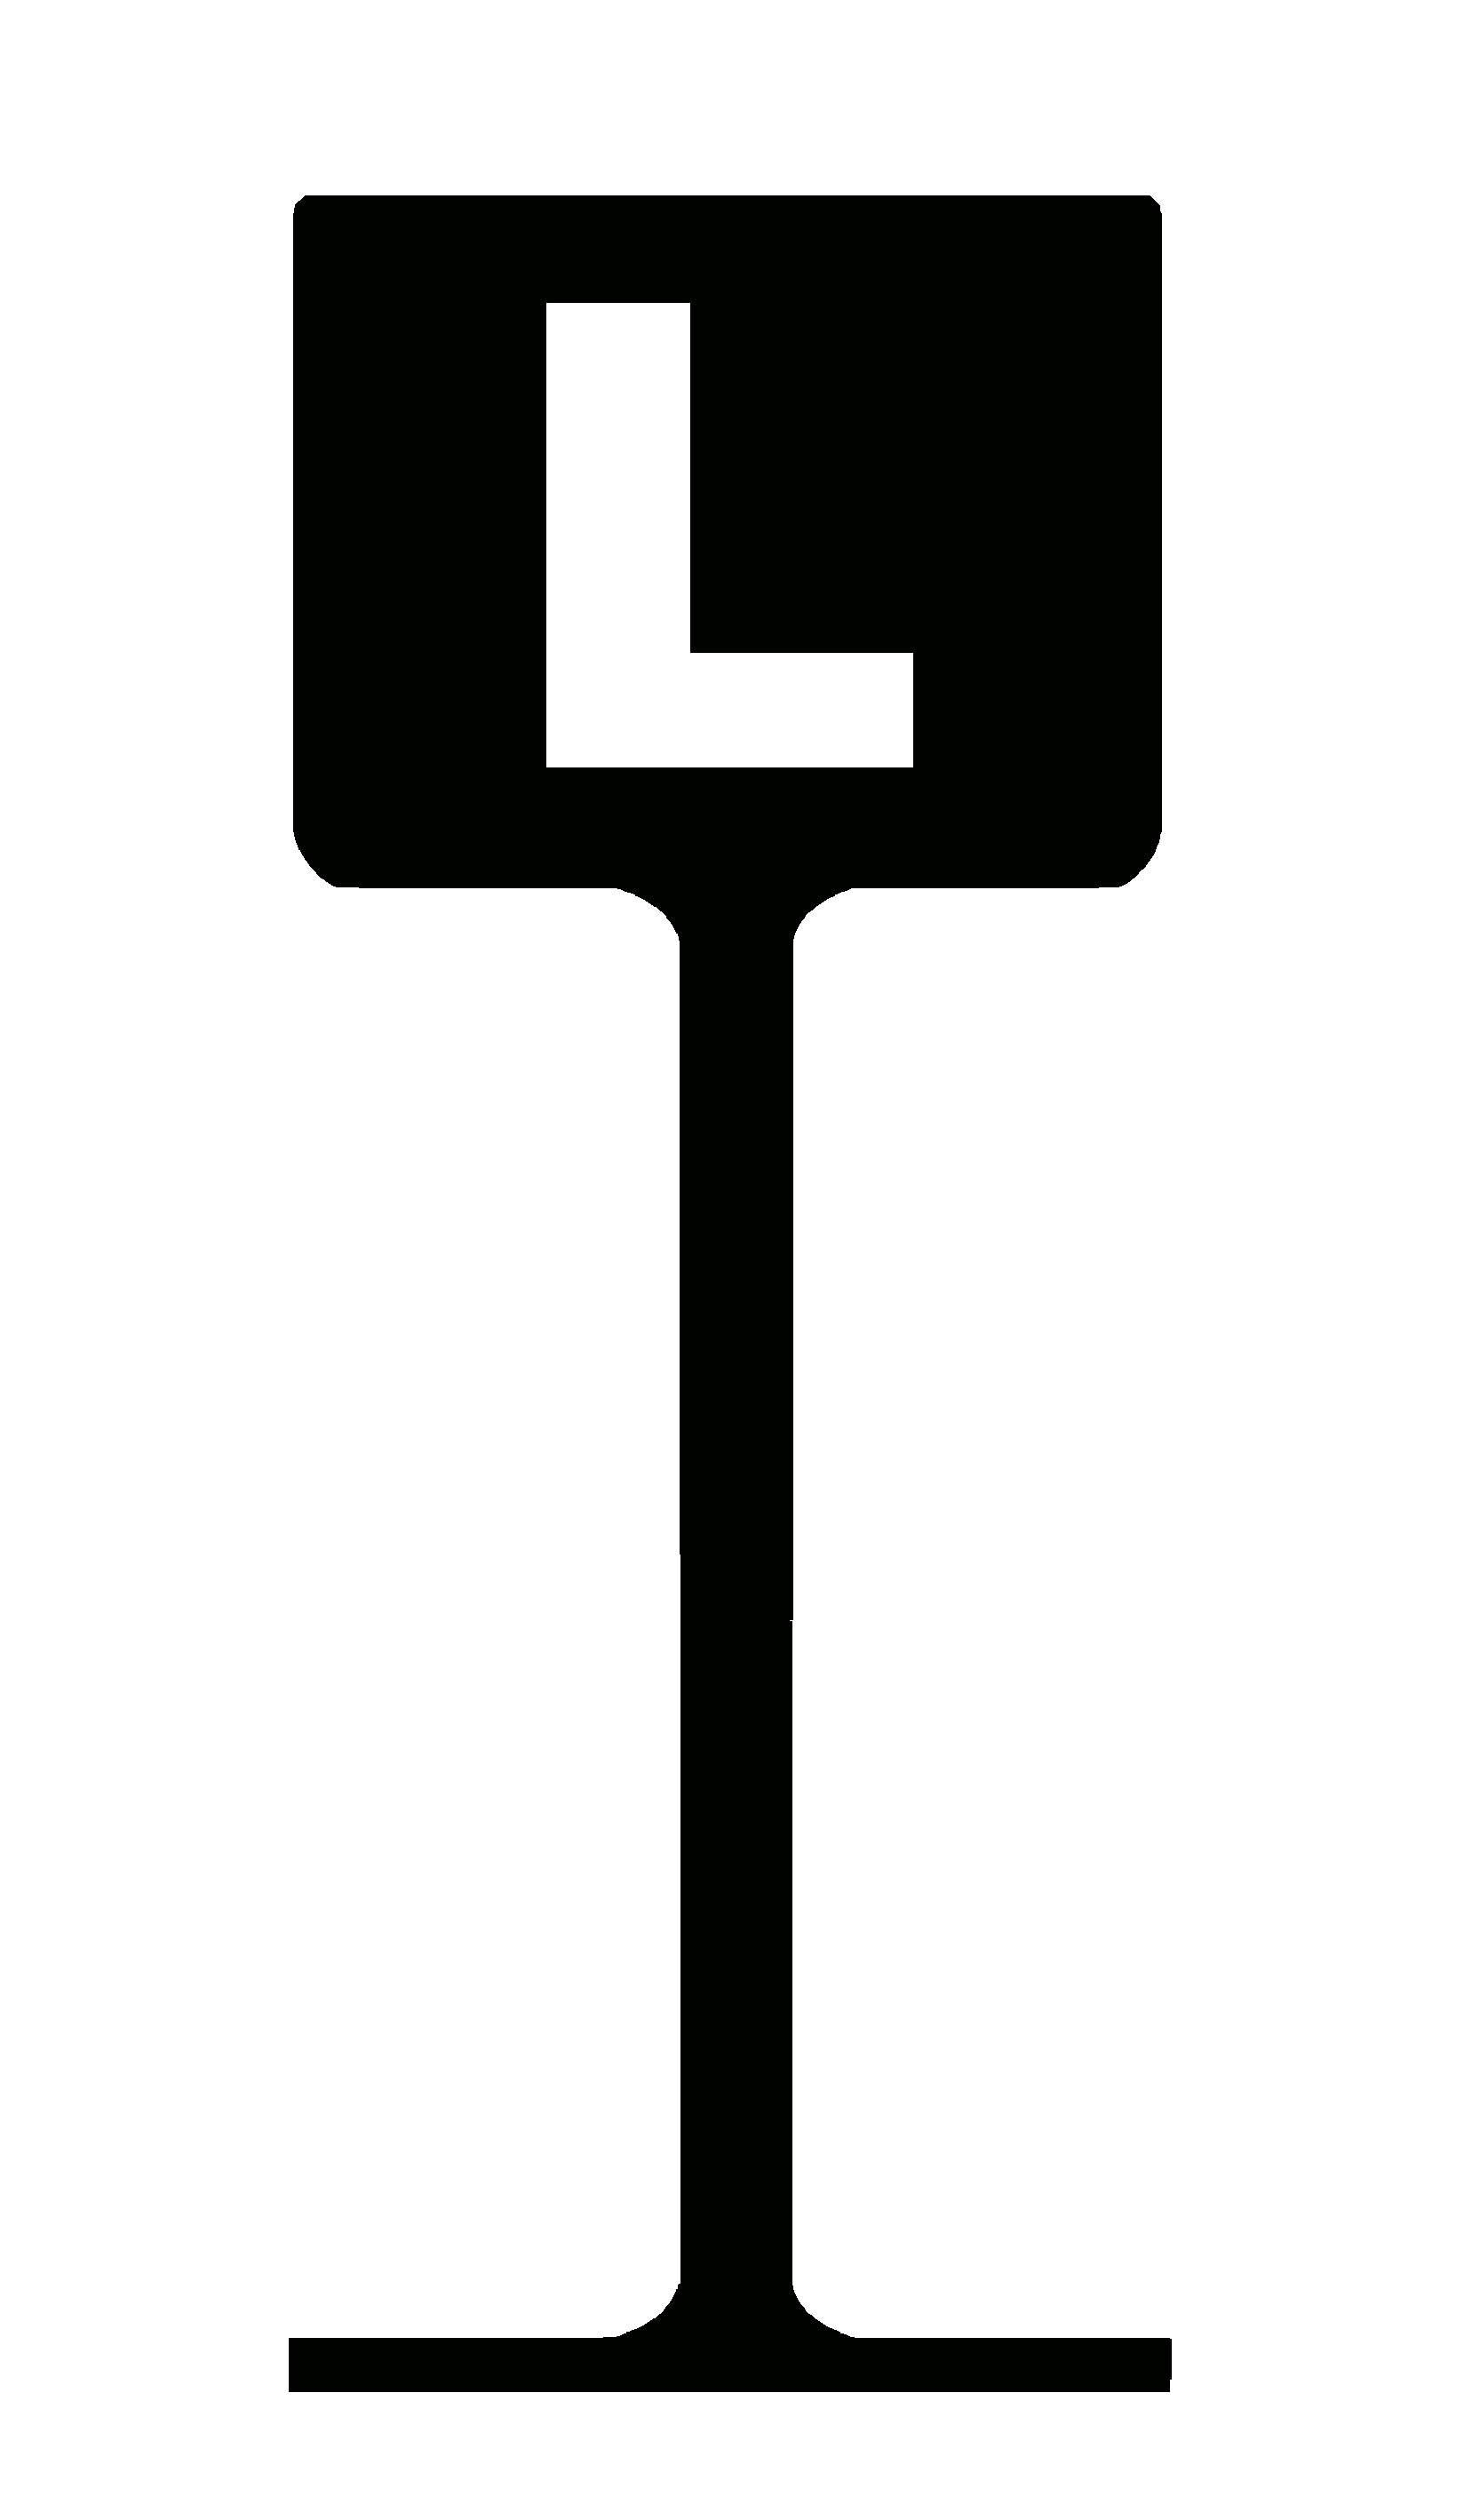
\includegraphics[scale=0.021, trim= 0em -5em -5em -5em,]{Icones/icon_loire_black.pdf}}}
	\parbox{\wd0}{\box0}
	& \quad Vallée de la Loire  & 
\setbox0=\hbox{\put(0,0){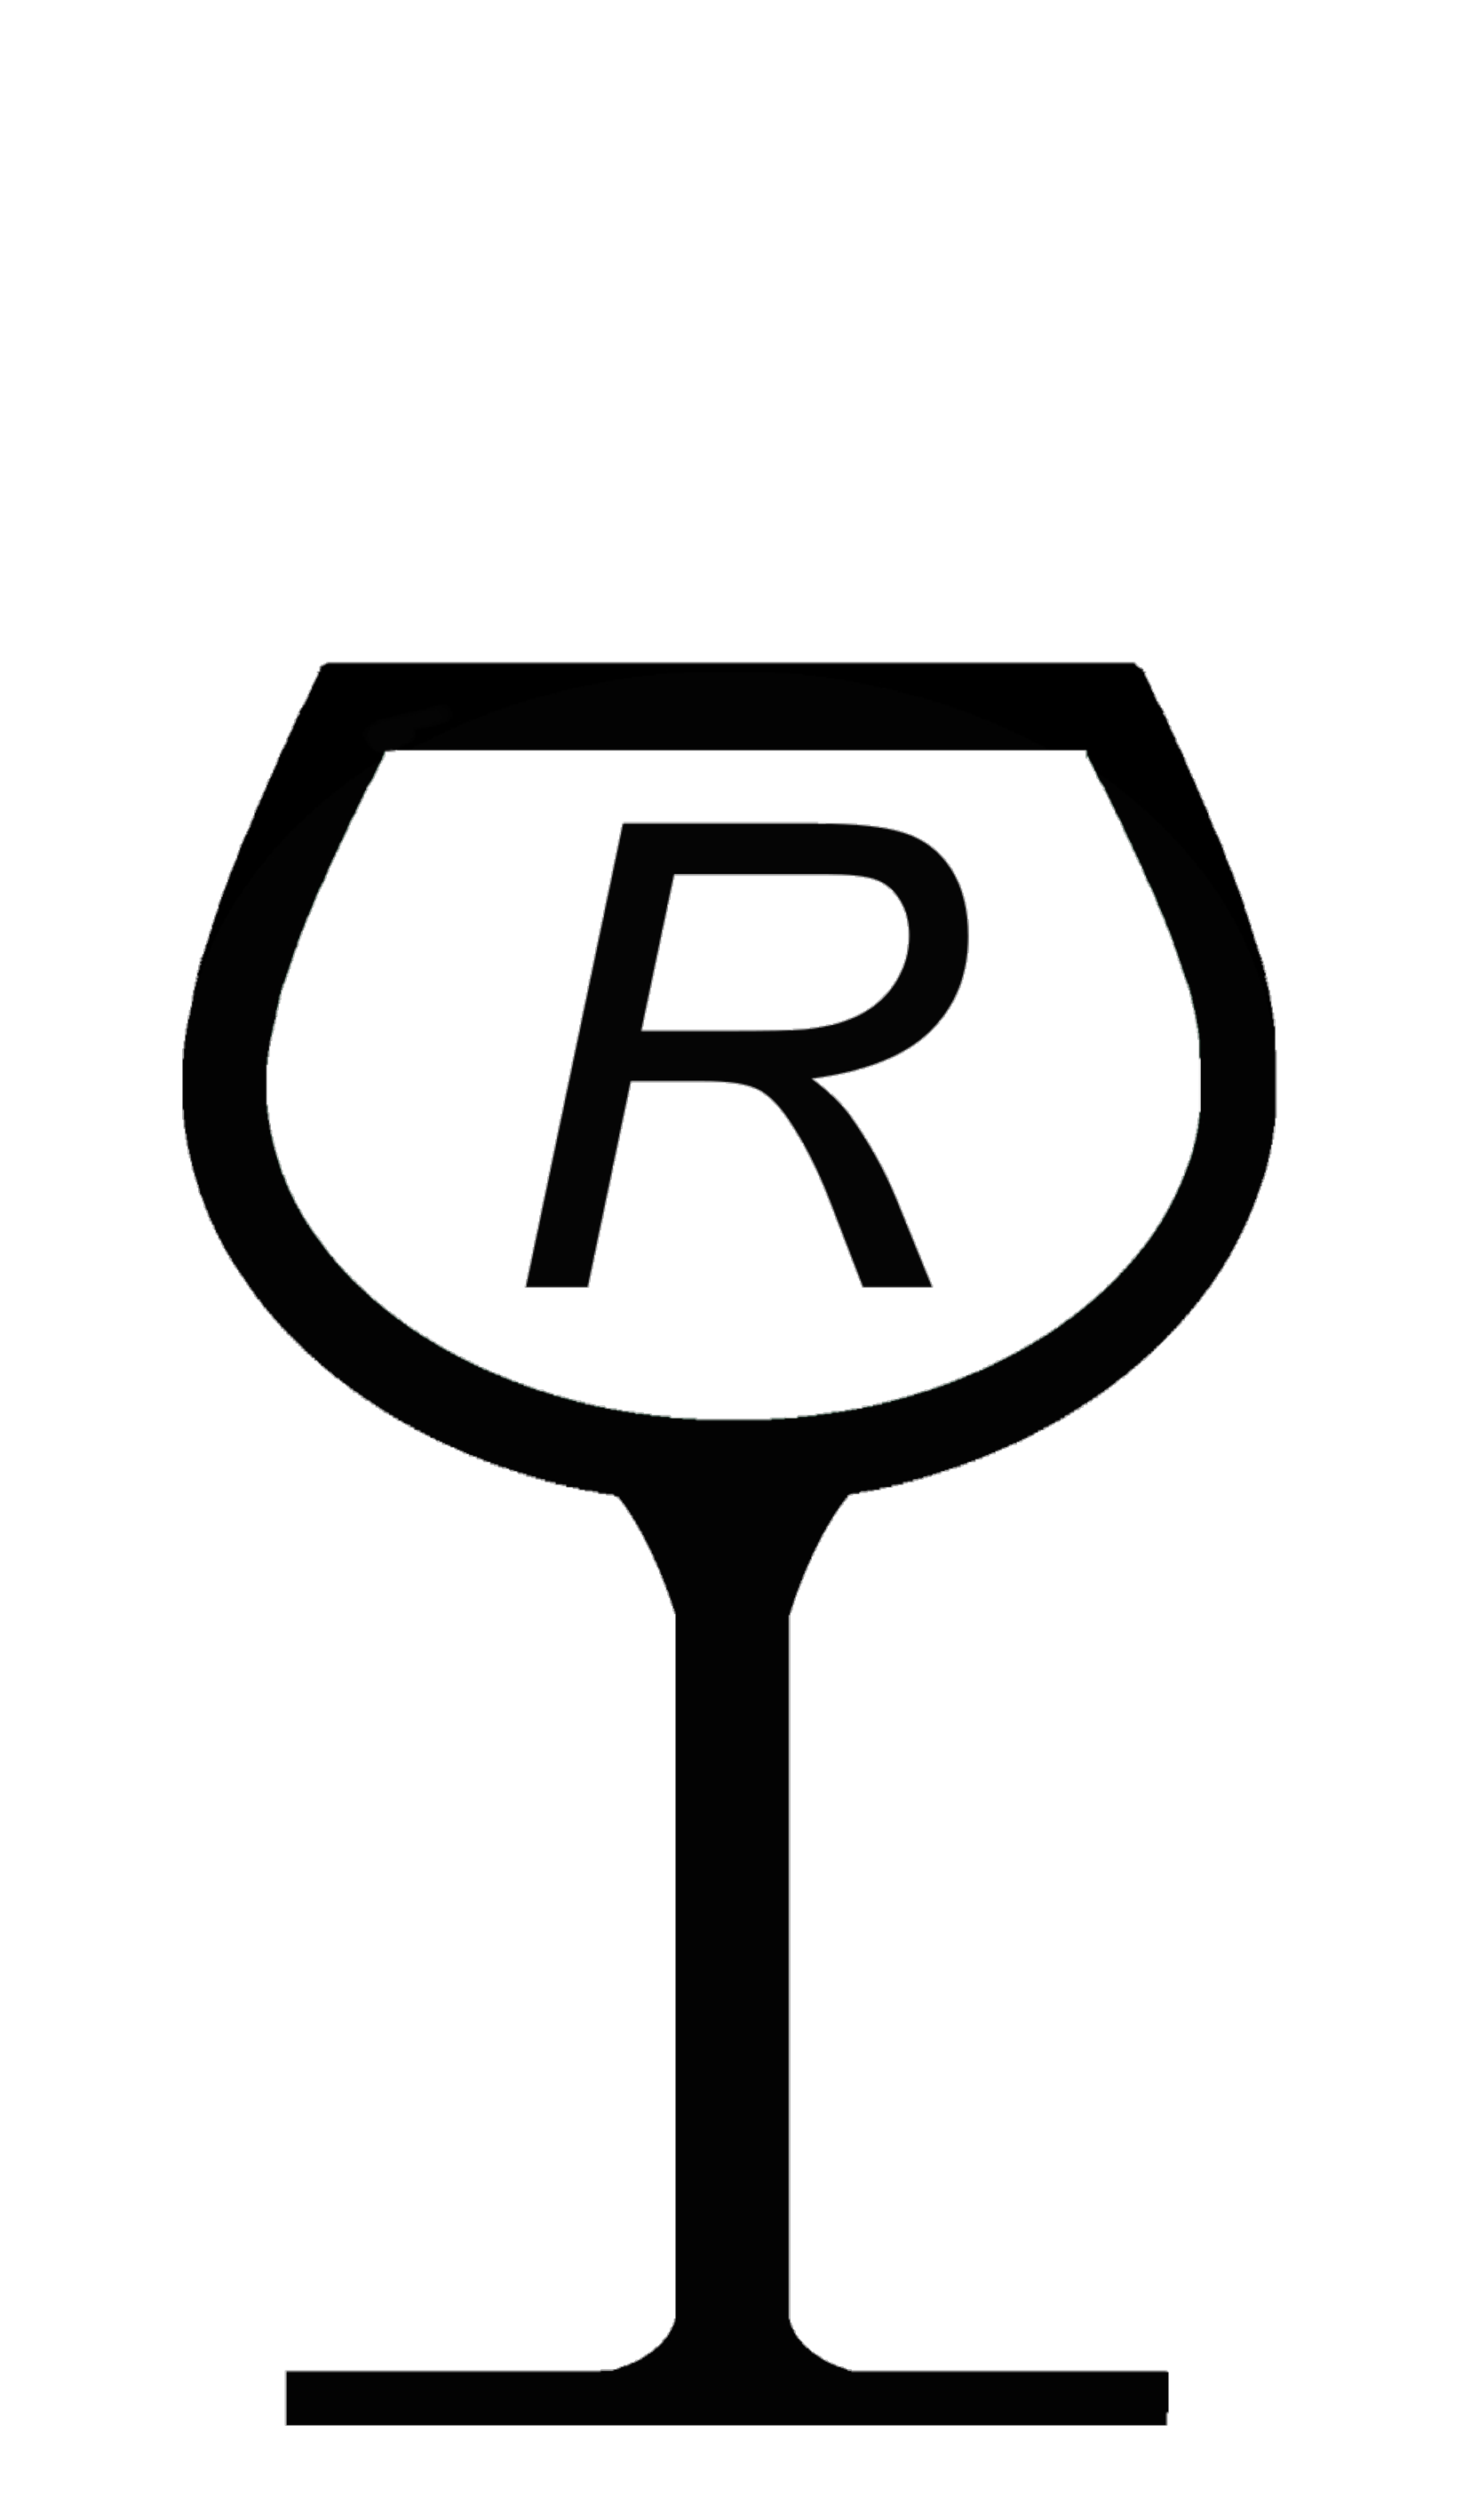
\includegraphics[scale=0.021, trim= 0em -5em -5em -5em,]{Icones/icon_rhone_black.pdf}}}
	\parbox{\wd0}{\box0}
	& \quad Vallée du Rhône  \\ 
\end{tabular}
\end{center}
}
\medskip
Tous les vins ont un pied pour que la température du vin ne soit pas modifiée par la main. Plus le vin doit resté frais, plus le pied est haut et le réservoir petit (Alsace, Loire, Champagne). Pour les vins qui ont en majorité des arômes légers qui s'évaporent vites (vins jeunes, Bourgogne), le bord doit être resserré. pour les vins qui ont en majorité des arômes lourds (vieux vins, Bordeaux, Rhône), le fond doit être rond et le bord plus large pour favoriser l'oxygénation qui fait remonter les arômes.

carte AOP

AOP c'est le nouveau label europeen qui doit remplacer AOC

\begin{figure}[t]
\includegraphics[width=\textwidth]{/home/paugam/Dropbox/CarteVin/maps/bassinViticoleFrance.png}
\end{figure}
\newpage
XX


